\section{Installation of Raspberry Pi OS}	\label{sec:run-raspberry}
	To install Raspberry Pi OS on ``Raspberry Pi 4 from CanaKit'', you will need to download \textbf{`Raspberry Pi Imager'} from the website. \href{https://www.raspberrypi.com/software}{here}. The \textbf{`Raspberry Pi Imager'} is supported by all OS (Mac/Windows/Linux). 
	
	\subsection{Installation of Raspberry Pi Imager on Mac}
		\begin{itemize}[leftmargin=1.7cm]
			\item[\textbf{Step 1:}] Download Raspberry Pi Imager from \href{https://downloads.raspberrypi.org/imager/imager_latest.dmg}{here}
			\item[\textbf{Step 2:}] Open/Install ``imager\_x.x.x.dmg''
			\item[\textbf{Step 3:}] Run application "Raspberry Pi Imager"\\
				\begin{minipage}{\textwidth}
					\vspace{2mm}
					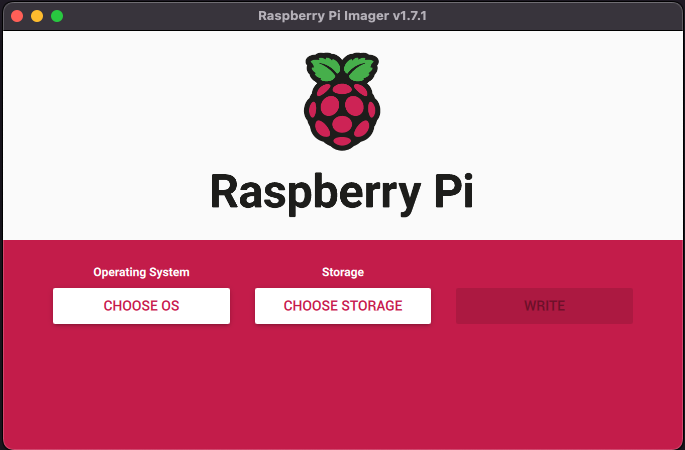
\includegraphics[scale=0.29]{Images/raspberry_pi/app.png}
					\vspace{2mm}
				\end{minipage}
			\item[\textbf{Step 4:}] Click on ``CHOOSE OS'' and Select \textbf{``Raspberry Pi OS (32-bit) Desktop''}\\
				\begin{minipage}{\textwidth}
					\vspace{2mm}
					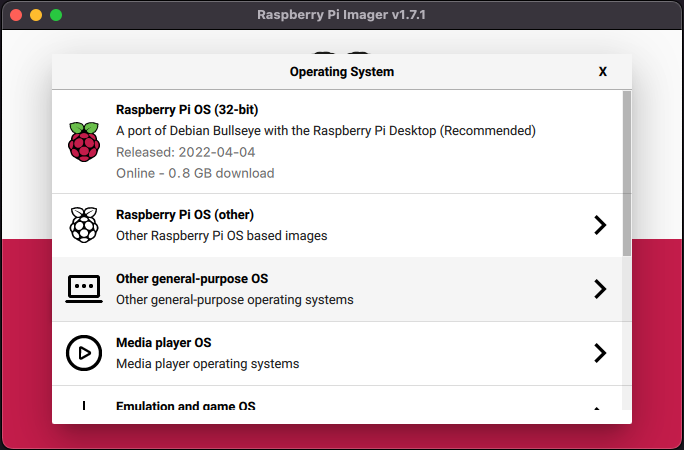
\includegraphics[scale=0.29]{Images/raspberry_pi/choose-os.png}
					\vspace{2mm}
				\end{minipage}
			\item[\textbf{Step 5:}] Click on ``CHOOSE STORAGE'' (\textbf{NOTE:} Please make sure you select correct SD card with is in Raspberry Pi 4)
			\item[\textbf{Step 6:}] Click on ``WRITE''
			\item[\textbf{Step 7:}] Wait untill writting is complete.
		\end{itemize}
	
	\subsection{Login to Raspberry Pi OS}
		At the begining  the user name of the OS is \textbf{``pi''} and password is \textbf{``raspberry''}. (\textbf{NOTE:} For this project we did \textbf{NOT} change any default user and password.)
	
	\subsubsection{Accessing Raspberry Pi}	\label{subsubsec:ssh}
		There are multiple ways you can access the \textbf{``pi''} user.  
		\begin{itemize}[leftmargin=1.2cm]
			\item Accessing through SSH \\
				To access \textbf{``pi''} user using SSH connection you need to make sure that your computer and Raspberry Pi are in same Internet connection. In this project it is ``eduroam'' connection. To setup ``eduroam'' connection into your newly install Raspberry Pi OS, please follow the instruction from \hyperref[sec:run-eduroam]{Appendix \ref{sec:run-eduroam}}.
				\begin{itemize}[leftmargin=1.3cm]
					\item[\textbf{Step 1:}] Open Terminal in your local computer \\
						\begin{minipage}{\textwidth}
							\vspace{2mm}
							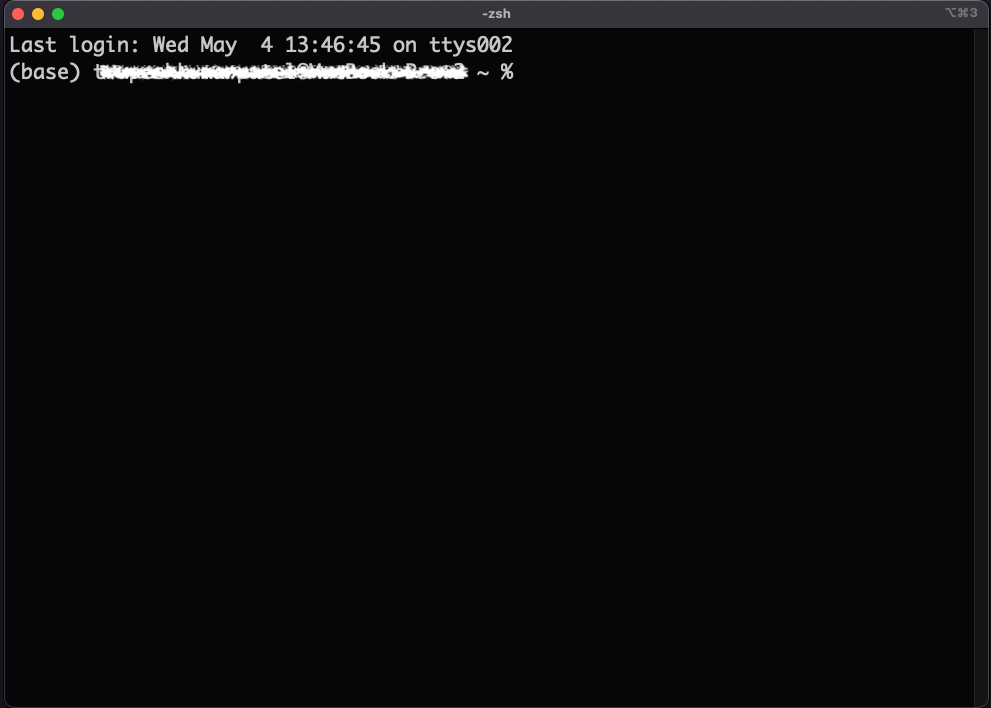
\includegraphics[scale=0.18]{Images/raspberry_pi/ssh_login/open_iterm.png}
							\vspace{2mm}
						\end{minipage}
					\item[\textbf{Step 2:}] Type command ``{\fontfamily{cmtt}\selectfont{ssh pi@10.127.227.11\\2}}'' <-- here `10.127.227.112' is IP address of Raspberry Pi, in your case might be different.\\
						\begin{minipage}{\textwidth}
							\vspace{2mm}
							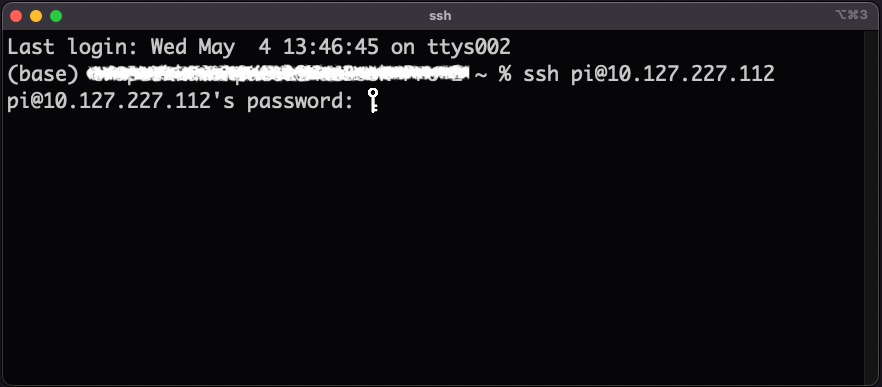
\includegraphics[scale=0.205]{Images/raspberry_pi/ssh_login/login.png}
							\vspace{2mm}
						\end{minipage}
					\item[\textbf{Step 3:}] Enter the password ``{\fontfamily{cmtt}\selectfont{raspberry}}''. Please enter the password that you set if you have, else it is going to be same as the authors.\\
						\begin{minipage}{\textwidth}
							\vspace{2mm}
							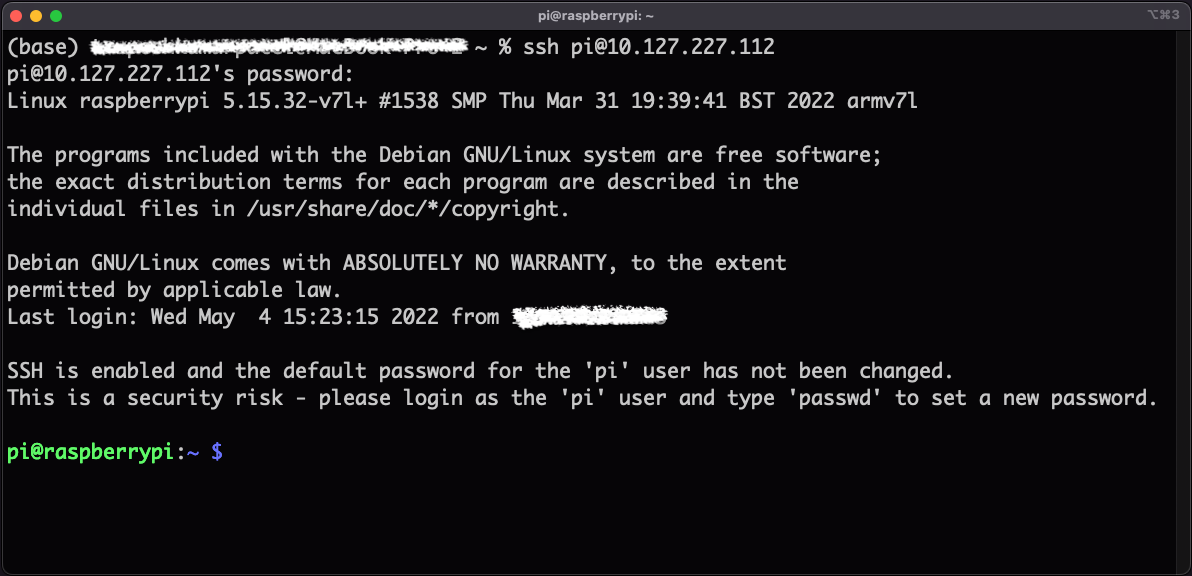
\includegraphics[scale=0.15]{Images/raspberry_pi/ssh_login/after_login.png}
							\vspace{2mm}
						\end{minipage}
				\end{itemize}
		\end{itemize}